\documentclass[ngerman, table, 9pt]{beamer}
\usetheme{metropolis}

%\usepackage[all]{hypcap}
\usepackage{colortbl}
\usepackage{scrhack}
\usepackage[utf8]{inputenc}

% Fira Sans
\usepackage[sfdefault]{FiraSans} %% option 'sfdefault' activates Fira Sans as the default text font
\usepackage[T1]{fontenc}
\renewcommand*\oldstylenums[1]{{\firaoldstyle #1}}

\usepackage[no-math]{fontspec}
\usepackage{babel}
%\usepackage[pdfborder={0 0 0}]{hyperref}
%\usepackage{amsmath}
\usepackage{adjustbox}
\usepackage{graphicx}
%\usepackage{float}
%\usepackage{amsfonts}
%\usepackage{textcomp}

% REFERENCE: https://www.ctan.org/tex-archive/macros/latex/contrib/drawstack
%\usepackage[nocolor]{drawstack}

\usepackage[backend=biber,style=alphabetic,sorting=ynt]{biblatex}
\addbibresource{deps/paper/bibliography.bib}

% JetBrains Mono
\setmonofont[Scale=MatchLowercase]{JetBrains Mono NL}

% \setlength{\parindent}{0pt}
\setlength{\parskip}{4pt}

\usepackage[autostyle]{csquotes}

\newcommand{\TODO}[1]{\textcolor{red}{\textbf{TODO: #1}}}
\newcommand{\rushCommit}{\ignorespaces\texttt{\input "|git -C ./deps/rush rev-parse --short HEAD"}\unskip}
\newcommand{\tokei}[1]{\input "|python3 tokei.py #1"}
\newcommand{\riscv}{RISC\babelhyphen{nobreak}V}

\newcommand{\qVerb}[2][]{`\Verb[#1]{#2}'}
\newcommand{\VerbCmd}[2][]{\Verb[commandchars=\\\{\}, #1]{#2}}
\newcommand{\qVerbCmd}[2][]{\qVerb[commandchars=\\\{\}, #1]{#2}}
\newcommand{\reg}[1]{\VerbCmd{\%#1}}
\newcommand{\qreg}[1]{\qVerbCmd{\%#1}}

% TODO: remove this command
\newcommand{\buildDate}{\ignorespaces\textcolor{red}{Timestamp: \texttt{\input "|date"} | Commit: \paperCommit}\unskip}

% \setcounter{tocdepth}{3}% Include \subsubsection in ToC

\newcounter{chapter}
\setcounter{chapter}{1}

\newcommand{\scite}[2][]{\footnotesize\cite[#1]{#2}}

\usepackage{tabularx}
\usepackage{multirow}
\usepackage{makecell}
\renewcommand{\arraystretch}{1.2}
\newcolumntype{L}{X}
\newcolumntype{C}{>{\centering\arraybackslash}X}
\newcolumntype{R}{>{\raggedleft\arraybackslash}X}

% ============================================================= %
% ==== FIXES and additionns for the `drawstack.sty` package === %
% ============================================================= %

% FEAT: Slight variation of the `\cellptr` command.
% The output of this command has a longer arrow with a steeper angle
\newcommand{\cellptrA}[1]{
	\draw[<-,line width=0.7pt] (0.1,\value{cellnb}) +(2,\value{ptrnb}*0.1) -- +(3.4,\value{ptrnb}*0.55);
	\draw (3.5,\value{ptrnb}*0.5+\value{cellnb}) node[anchor=west] {#1};
	\addtocounter{ptrnb}{1}
}

% TODO: decide whether the colors of the stack should be customized
%\tikzstyle{freecell}=[fill=gray!10]
%\tikzstyle{occupiedcell}=[fill=gray!10!orange!10,draw=blue!30!black]
%\tikzstyle{padding}=[fill=yellow!20,draw=blue!30!black]
%\tikzstyle{highlight}=[draw=orange!50!black,text=orange!50!black]

% HACK: These two commands are required in order to allow cell pointers targeing the stacktop
\newcommand{\llcellFixed}[3]{
    \addtocounter{cellnb}{-#1}
    \setcounter{ptrnb}{0}
    \draw[#2] (0,\value{cellnb})
    +(-2,.5) -- +(-2,-.5) -- +(2,-.5) -- +(2,.5);
    \draw (0,\value{cellnb}+#1/2-0.5)  node(currentcell) {#3};
}

\newcommand{\stackTopFixed}[2][freecell]{%
\llcellFixed{1}{#1}{#2}}

% HACK: redefine `\finishframe` to adjust the horizontal label spacing
\renewcommand{\finishframe}[1]{
  \draw[snake=brace, line width=0.6pt, segment amplitude=7pt]
  (-2,\value{cellnb}-0.5) -- (-2,\value{startframe}-0.5);
  \draw (-4.65cm,\value{cellnb}*0.5+\value{startframe}*0.5-0.5) node
  {\parbox{3cm}{%
\begin{flushright}
#1
\end{flushright}}};
}


\input{|"lirstings include-tex"}
\captionsetup{labelformat=empty}
% Set `deps/rush` as path prefix in all lirstings, is ignored for files under other directories
\NewCommandCopy{\oldLirsting}{\Lirsting}
\renewcommand{\Lirsting}[2][]{\oldLirsting[path prefix={deps/rush},vspace=0pt,#1]{#2}}

\usepackage{tikz}
\usepackage{nicematrix}
\usetikzlibrary{arrows.meta,shapes.geometric, shapes.multipart, fit, positioning, trees}

\tikzstyle{rec} = [rectangle, minimum width=3cm, minimum height=1cm,text centered, draw=black]
\tikzstyle{arrow} = [thick,->,>=stealth]

\tikzstyle{vstack} = [
rectangle split,
rectangle split parts=#1,
draw,
anchor=center,
]
\tikzstyle{stack} = [
rectangle split horizontal,
rectangle split part align=base,
vstack=#1,
]

% For the linker Figure
\tikzstyle{center} = [ellipse, rounded corners, minimum width=2cm, minimum height=1.25cm,text centered, draw=black, fill=gray!30]
\tikzstyle{entity} = [rectangle, minimum width=3cm, minimum height=1cm, text centered, align=center, draw=black, fill=gray!10]
\tikzstyle{relation} = [arrow, shorten >= 3pt, shorten <= 3pt]

% For the CPU - register - memory Figure
\tikzstyle{darrow} = [arrow, <->, shorten >= 3pt, shorten <= 3pt]


\title{Die Umwandlung von Quelltext in Maschinensprache}
\date{17. Mai 2023}
\author{Silas Groh, Mik Müller}
\institute{Carl-Fuhlrott-Gymnasium}

\titlegraphic{\rushlogo{y=0.80pt, x=0.80pt, yscale=-0.17, xscale=0.17}}

\begin{document}
\begin{frame}
	\titlepage
\end{frame}

\section{Einstieg \& Motivation}
\begin{frame}{Einstieg \& Motivation}
	\begin{itemize}
		\item Computerprogrammer werden oft in speziell entwickelten Programmiersprachen verfasst
		\item Vorteile eines hohen Abstraktionsgrades~\scite[S.~9]{Dandamudi2005Risc}:
		      \begin{itemize}
			      \item Entwicklung ist einfacher und schneller
			      \item Programme sind portabel
			      \item Instandhaltung ist einfacher
		      \end{itemize}
	\end{itemize}
\end{frame}

\begin{frame}{Zentrales Problem}
	\begin{minipage}{.35\textwidth}
		\Lirsting[float=H, fancyvrb={frame=none}, size=small]{deps/paper/listings/simple.rush}
	\end{minipage}%
	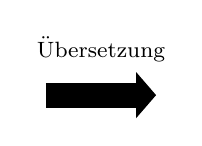
\begin{tikzpicture}[triangle/.style={-{Triangle[width=\the\dimexpr1.8\pgflinewidth,length=\the\dimexpr0.8\pgflinewidth]}}]
		\draw[line width=9pt,triangle](0,0) -- node[anchor=south, yshift=.15cm] {\footnotesize Übersetzung} (1.4,0);
	\end{tikzpicture}
	\hfill
	\begin{minipage}{.35\textwidth}
		\Lirsting[float=H, fancyvrb={frame=none}, ranges={1-10}, size=small]{listings/generated/rush_simple.hexdump}
	\end{minipage}

	\begin{itemize}
		\item Programme sollten einfach zu schreiben sein
		\item[\Rightarrow] Ein Computer muss diese jedoch auch \textit{einfach} verarbeiten
	\end{itemize}
\end{frame}

\begin{frame}{Methoden zur Programmausführung}
	\begin{itemize}
		\item Man unterscheidet zwischen \emph{Compilern} und \emph{Interpretern}
		\item Ein Compiler (auch \emph{Übersetzer}) übersetzt die Sprache in ein zielspezifiesches Format, sodass ein Computer dieses verstehen kann
		\item Ein Interpreter führt das Programm direkt aus, ohne es vorher zu bearbeiten
	\end{itemize}
\end{frame}

\begin{frame}{Etappen der Übersetzung}
	\begin{figure}[h]
		\begin{adjustbox}{max totalsize={\textwidth}{!},center}
			
\begin{tikzpicture}[node distance=1cm, inner sep=3mm]
				\node (lexical_analysis) [rec, minimum height=1.5cm] {Lexikalische Analyse};
				\node (syntactic_analysis) [rec, right=of lexical_analysis, align=center, minimum height=1.5cm] {Syntaxanalyse};
				\draw [arrow] (lexical_analysis) -- (syntactic_analysis);
				\node (semantic_analysis) [rec, right=of syntactic_analysis, align=center, minimum height=1.5cm] {Semantische\\Analyse};
				\draw [arrow] (syntactic_analysis) -- (semantic_analysis);
				\node (codegen) [rec, right=of semantic_analysis, minimum height=1.5cm] {Code-Erzeugung};
				\draw [arrow] (semantic_analysis) -- (codegen);
			\end{tikzpicture}
		\end{adjustbox}
		\caption{Etappen der Übersetzung}{\scite[S.~6--7]{wirth_compiler_construction_2005}}\label{fig:compilation_steps}
	\end{figure}
\end{frame}

\begin{frame}{Etappen der Übersetzung (angepasst)}
	\begin{figure}[h]
		\begin{adjustbox}{max totalsize={\textwidth}{!},center}
			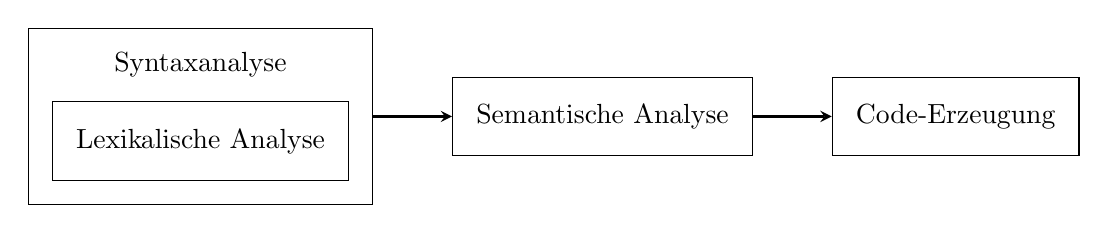
\begin{tikzpicture}[node distance=3mm and 1cm, inner sep=3mm]
				\node (syntactic_analysis_text) [inner sep=0] {Syntaxanalyse};
				\node (lexical_analysis) [rec, below=of syntactic_analysis_text] {Lexikalische Analyse};
				\node (syntactic_analysis) [rec, fit={(syntactic_analysis_text) (lexical_analysis)}] {};
				\node (semantic_analysis) [rec, right=of syntactic_analysis] {Semantische Analyse};
				\draw [arrow] (syntactic_analysis) -- (semantic_analysis);
				\node (codegen) [rec, right=of semantic_analysis] {Code-Erzeugung};
				\draw [arrow] (semantic_analysis) -- (codegen);
			\end{tikzpicture}
		\end{adjustbox}
		\caption{Etappen der Übersetzung (angepasst)}{\scite[S.~6--7]{wirth_compiler_construction_2005}}\label{fig:compilation_steps_altered}
	\end{figure}
\end{frame}

\subsection{Die Programmiersprache \enquote{rush}}

\begin{frame}{Die Programmiersprache \enquote{rush}}
	\center
	\begin{minipage}{.95\textwidth}
		\Lirsting[caption={Erzeugen von Fibonaccizahlen in rush}, label={lst:rush_fib}, float=H]{deps/paper/listings/fib.rush}
	\end{minipage}
\end{frame}

\begin{frame}{Fähigkeiten von rush}
	\begin{table}[h]
		\caption{Die wichtigsten Fähigkeiten von rush}\label{tbl:rush_features}
		\rowcolors{2}{gray!15}{}
		\begin{tabularx}{0.95\textwidth}{Ll}
			\rowcolor{gray!25} Bezeichnung & rush Ausdruck                                     \\
			\hline
			Loop                           & \LirstInline{rush}{loop {  }}                     \\
			While                          & \LirstInline{rush}{while x < 5 {  }}              \\
			For                            & \LirstInline{rush}{for i = 0; i < 5; i += 1 {  }} \\
			If                             & \LirstInline{rush}{if true { /* */ } else {  }}   \\
			Fn                             & \LirstInline{rush}{fn foo(n: int) {  }}           \\
			Infix Expr                     & \LirstInline{rush}{1 + n; 5 ** 2}                 \\
			Prefix Expr                    & \LirstInline{rush}{!false; -n}                    \\
			Variables                      & \LirstInline{rush}{let mut answer = 42}           \\
			Cast Expr                      & \LirstInline{rush}{42 as char}                    \\
		\end{tabularx}
	\end{table}
\end{frame}

\begin{frame}{Datentypen in rush}
	\begin{table}[h]
		\caption{Datentypen in rush}\label{tbl:rush_types}
		\rowcolors{2}{gray!15}{}
		\begin{tabularx}{0.95\textwidth}{lL}
			\rowcolor{gray!25} Bezeichnung & Instanziierung einer Variable            \\
			\hline
			\qVerb{int}                    & \LirstInline{rush}{let a: int = 0;}      \\
			\qVerb{float}                  & \LirstInline{rush}{let b: float = 3.14;} \\
			\qVerb{bool}                   & \LirstInline{rush}{let c: bool = true;}  \\
			\qVerb{char}                   & \LirstInline{rush}{let d: char = 'a';}   \\
			\qVerb{()}                     & \LirstInline{rush}{let e: () = main();}  \\
			\qVerb{!}                      & \LirstInline{rush}{let f = exit(42);}    \\
		\end{tabularx}
	\end{table}
\end{frame}

\begin{frame}{Fakten über rush}
	\begin{itemize}
		\item Im Commit \rushCommit~umfasste das Projekt \rushLoc~Zeilen Programmtext\footnote{Leerzeilen und Kommentare werden nicht gezählt}
		\item Das Projekt enthält einen Lexer, einen Parser, fünf Compiler und einen Interpreter
	\end{itemize}
\end{frame}

\begin{frame}{Programmtext der einzelnen Komponenten}
	\begin{table}[h]
		\centering
		\caption{Zeilen Programmtext pro Komponente}\label{tbl:rush_loc_components}
		\begin{tabularx}{0.95\textwidth}{|L|L|}
			\hline
			\rowcolor{gray!20} Komponente & Zeilen Programmtext                                                  \\ \hline
			Lexer / Parser                & \tokei{./deps/rush/crates/rush-parser}                               \\ \hline
			Tree-walking interpreter      & \cellcolor{gray!15} \tokei{./deps/rush/crates/rush-interpreter-tree} \\ \hline
			VM compiler / runtime         & \tokei{./deps/rush/crates/rush-interpreter-vm}                       \\ \hline
			WASM compiler                 & \tokei{./deps/rush/crates/rush-compiler-wasm}                        \\ \hline
			LLVM compiler                 & \cellcolor{gray!15} \tokei{./deps/rush/crates/rush-compiler-llvm}    \\ \hline
			RISC-V compiler               & \tokei{./deps/rush/crates/rush-compiler-risc-v}                      \\ \hline
			x86 compiler                  & \cellcolor{gray!15} \tokei{./deps/rush/crates/rush-compiler-x86-64}  \\ \hline
		\end{tabularx}
	\end{table}
\end{frame}

\section{Lexikalische \& Syntaktische Analyse}
\begin{frame}{Lexikalische \& Syntaktische Analyse}
	Hello, world!
	\cite{Jeffery2021}
	\cite{Watson2017}
	\cite{Sendil2022-fy}
\end{frame}

% LTeX: language=de-DE
\section{Semantische Analyse}

\begin{frame}{Etappen der Übersetzung: Semantische Analyse}
	\begin{figure}[h]
		\begin{adjustbox}{max totalsize={\textwidth}{!},center}
			\begin{tikzpicture}[node distance=1cm, inner sep=3mm]
				\node (lexical_analysis) [rec, minimum height=1.5cm] {Lexikalische Analyse};
				\node (syntactic_analysis) [rec, right=of lexical_analysis, align=center, minimum height=1.5cm] {Syntaxanalyse};
				\draw [arrow] (lexical_analysis) -- (syntactic_analysis);
				\node (semantic_analysis) [rec, right=of syntactic_analysis, align=center, minimum height=1.5cm, fill=mLightBrown!35] {Semantische\\Analyse};
				\draw [arrow] (syntactic_analysis) -- (semantic_analysis);
				\node (codegen) [rec, right=of semantic_analysis, minimum height=1.5cm] {Code-Erzeugung};
				\draw [arrow] (semantic_analysis) -- (codegen);
			\end{tikzpicture}
		\end{adjustbox}
	\end{figure}
\end{frame}

\begin{frame}{Semantische Analyse \& Semantikregeln}
	\begin{itemize}
		\item Validiert die semantische Eigenschaften
		\item Meistens: Definition in einer natürlichen Sprache
	\end{itemize}
\end{frame}

\begin{frame}{Beispiel 1: Invalides rush Programm}
	\begin{minipage}{.5\textwidth}
		\Lirsting[float=H, fancyvrb={frame=none}]{listings/incompatible_types.rush}
	\end{minipage}%
	\begin{minipage}{.5\textwidth}
		\Darrow{Fehlerausgabe}
	\end{minipage}
	\Lirsting[float=H, fancyvrb={frame=none, fontsize=\footnotesize}, ansi=true]{listings/generated/incompatible_types.rush.out}
\end{frame}

\begin{frame}{Beispiel 2: Invalides rush Programm}
	\begin{minipage}{.5\textwidth}
		\Lirsting[float=H, fancyvrb={frame=none}]{listings/invalid_main_fn.rush}
	\end{minipage}%
	\begin{minipage}{.5\textwidth}
		\Darrow{Fehlerausgabe}
	\end{minipage}
	\Lirsting[float=H, fancyvrb={frame=none, fontsize=\footnotesize}, ansi=true]{listings/generated/invalid_main_fn.rush.out}
\end{frame}

\begin{frame}{Beispiel 3: Warnung aufgrund einer unbenutzten Variable}
	\begin{minipage}{.5\textwidth}
		\Lirsting[float=H, fancyvrb={frame=none}]{listings/unused_var.rush}
	\end{minipage}%
	\begin{minipage}{.5\textwidth}
		\Darrow{Ausgabe}
	\end{minipage}
	\Lirsting[float=H, fancyvrb={frame=none, fontsize=\footnotesize}, ansi=true]{listings/generated/unused_var.rush.out}
\end{frame}

\begin{frame}{Anforderungen an die semantische Analyse (für rush)}
	\begin{itemize}
		\item<1-> Unterscheidung zwischen validen und invaliden Programmen
		\item<2-> hilfreiche Warnungen und Informationen
		\item<3-> Hinzufügen von Typinformationen zu dem AST
		\item<4-> Triviale Optimierungen der Programmstruktur
	\end{itemize}
\end{frame}

\begin{frame}{Hinzufügen von Informationen über Datentypen}
	\begin{figure}[h]
		\begin{adjustbox}{max totalsize={\textwidth}{!},center}
			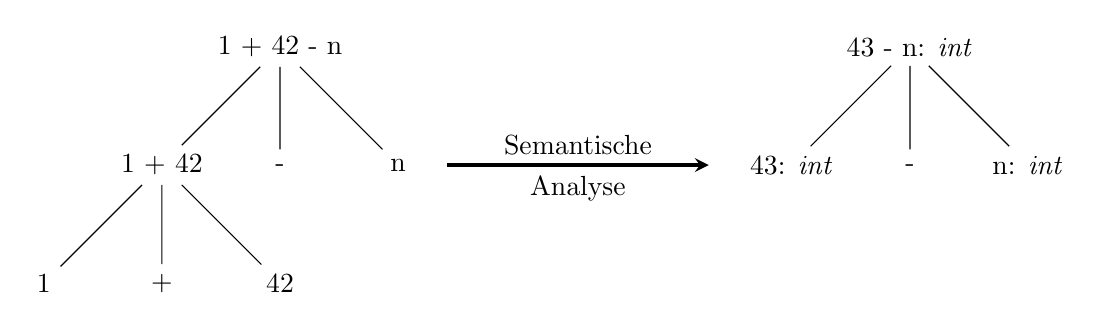
\begin{tikzpicture}[
					tlabel/.style={pos=0.4,right=-1pt,font=\footnotesize\color{red!70!black}},
				]
				\node(left){\Verb{1 + 42 - n}}
				child { node { \Verb{1 + 42} }
						child { node { \Verb{1} } }
						child { node { \Verb{+} } }
						child { node { \Verb{42} } }
					}
				child { node  { \Verb{-} }       }
				child { node(leftm)  { \Verb{n} } };

				\node(right)[right of=left, xshift=7cm]{\Verb{43 - n}: \emph{int}}
				child { node(rightm) { \Verb{43}: \emph{int} } }
				child { node  { \Verb{-} } }
				child { node  { \Verb{n}: \emph{int} } };

				\draw[arrow, shorten >= 0.4cm, shorten <= 0.4cm, very thick] (leftm) -- node[above] {Semantische} node[below] {Analyse} ++ (rightm);
			\end{tikzpicture}
		\end{adjustbox}
	\end{figure}
\end{frame}

\section{Interpreter}
\begin{frame}{Tree-walking Interpreter}
	\TODO{\@RubixDev Write this}
\end{frame}

% LTeX: language=de-DE

\pdfpcnote{
	@Mik \\
	\\
	- Zusaetzlich: wir haben eine **Virtuelle Maschine** implementiert \\
}
\section{Virtuelle Maschine}

\begin{frame}{Etappen der Übersetzung: Code-Erzeugung}
	\pdfpcnote{
		@Mik \\
		\\
		- Wichtig: erste Projekt, welches **Code-Erzeugung**; **einen Compiler** benoetigt \\
	}
	\begin{figure}[h]
		\begin{adjustbox}{max totalsize={\textwidth}{!},center}
			\begin{tikzpicture}[node distance=3mm and 1cm, inner sep=3mm]
				\node (syntactic_analysis_text) [inner sep=0] {Syntaxanalyse};
				\node (lexical_analysis) [rec, below=of syntactic_analysis_text] {Lexikalische Analyse};
				\node (syntactic_analysis) [rec, fit={(syntactic_analysis_text) (lexical_analysis)}] {};
				\node (semantic_analysis) [rec, right=of syntactic_analysis] {Semantische Analyse};
				\draw [arrow] (syntactic_analysis) -- (semantic_analysis);
				\node (codegen) [rec, fill=mLightBrown!35, right=of semantic_analysis] {Code-Erzeugung};
				\draw [arrow] (semantic_analysis) -- (codegen);
			\end{tikzpicture}
		\end{adjustbox}
	\end{figure}
\end{frame}

\begin{frame}{Virtuelle Maschine}
	\pdfpcnote{
		@Mik \\
		\\
		- Simuliert eine VM nicht einen ganzen Computer? \\
		- die CPU \\
		- das Display \\
		- und die Festplatte \\
		\\
		--- \\
		\\
		- Hier: **Software, die NUR wie die CPU eines Rechners funktioniert** \\

	}
	\begin{itemize}
		\item<1-> Häufig: Eine \emph{Virtuelle Maschine} (VM) simuliert echte Computer
			\begin{itemize}
				\item Display
				\item Lautsprecher
				\item Festplatte
				\item \dots
			\end{itemize}
		\item<2-> Hier: Software, die wie die CPU eines Rechners funktioniert
	\end{itemize}
\end{frame}

\begin{frame}{Virtuelle Maschine}
	\pdfpcnote{
		@Mik \\
		\\
		- Hier: Ablauf aehnelt dem des Compilers \\
		- Zuerst: Umwandlung in ein Format, welches die VM versteht \\
		- Diese fuehrt dieses dann aus \\
		\\
		--- \\
		\\
		- von Aussen: wie ein Schritt; Einordnung zu Interpretern\\
		- aehnlich: **Python** \\
	}

	\hspace{.3cm}
	\begin{minipage}{.2\textwidth}
		\begin{center}
			\Lirsting[float=H, fancyvrb={frame=none, fontsize=\footnotesize}]{deps/paper/listings/simple.rush}
		\end{center}
	\end{minipage}%
	\hspace{-.3cm}
	\Larrow{
		\begin{minipage}{1.3cm}
			Compiler
		\end{minipage}
		\begin{minipage}{5mm}
			
\includegraphics[width=3.5mm]{assets/google_icon_settings.png}
		\end{minipage}
	}
	\hspace{.8cm}
	\begin{minipage}{.24\textwidth}
		\Lirsting[float=H, fancyvrb={frame=none, fontsize=\footnotesize}, ranges={4-20}]{listings/simple_vm.s}
	\end{minipage}
	\Larrow{
		\begin{minipage}{.4cm}
			VM
		\end{minipage}
		\begin{minipage}{5mm}
			
\includegraphics[width=3.5mm]{assets/google_icon_settings.png}
		\end{minipage}
	}
	\hspace{.1cm}
	\begin{minipage}{.13\textwidth}
		\centering
		{\large Exit code: 5}
	\end{minipage}
	\hfill

	\begin{itemize}
		\item Python, usw.
		\item Umwandlung in ein anderes Format
		\item[\Rightarrow] Anschliessende Ausführung des Programmes
	\end{itemize}
\end{frame}

\begin{frame}{Die rush VM}
	\pdfpcnote{
		@Mik \\
		\\
		- Diese Konzepte wurden nun auch auf die rush VM uebertragen \\
		\\
		--- \\
		\\
		- 1 Ausfuehrung vorher uebersetzter Programme\\
		- 2 **eine selbst entwickelte Architektur**, die das Ziel des Compilers darstellt \\
		- **stackbasiertes Design**, **hoher Abstaktionsgrad**
	}
	\begin{itemize}
		\item<1-> Führt ein zuvor übersetztes Programm aus
		\item<2-> Besitzt eine selbst entwickelte Architektur
			\begin{itemize}
				\item Stackbasiertes Design
				\item Hoher Abstaktionsgrad
			\end{itemize}
	\end{itemize}
\end{frame}

\begin{frame}{Felder der VM}
	\pdfpcnote{
		@Mik \\
		\\
		- Vgl. Tree-walking Interpreter: die VM hat 4 Felder \\
		\\
		--- \\
		\\
		1. **stack** fuer temporaere Werte \\
		2. **mem** und **mem-ptr** zur Speicherung von Variablen \\
		3. **call-stack** (also Aufrufstapel): verwaltet mehrere **Befehlszaehler** und **Funktionszaehler** \\
	}
	\begin{description}
		\item<1->[stack] Für temporäre Werte
		\item<2->[mem] Für Variablen
		\item<2->[mem\_ptr] Für Speicherverwaltung
		\item<3->[call\_stack] Aufrufstapel (\emph{Befehlsähler} und \emph{Funktionszähler})
	\end{description}
\end{frame}

\begin{frame}{Struktur der Programme der rush VM}
	\pdfpcnote{
		@Mik \\
		\\
		- 1 Die Programme der VM sind in Funktionen aufgeteilt \\
		- keinen Namen aber numerische Identifizierung \\
		- Jede Funktion enthaehlt mehrere Anweisungen \\
		- 2 Als Beispiel betrachten wir die Anweisung **call 2** \\
		- Der Befehlscode, also **call** \\
		- Und ein optionaler Operand, hier die **2** \\
		- 3 gerade einmal ca. 30 verschiedene Befehlscodes \\
	}
	\begin{itemize}
		\item<1-> Unterteilung in Funktionen
			\begin{itemize}
				\item Ohne Namen
				\item Numerische Identifizierung
				\item Enthält mehrere Anweisungen
			\end{itemize}
		\item<2-> Struktur der Anweisungen: \enquote{\LirstInline{asm}{call 2}}
			\begin{itemize}
				\item<2-> Befehlscode (\texttt{call})
				\item<2-> Optionaler Operand (\texttt{2})
			\end{itemize}
		\item<3-> ca. 30 verschiedene Befehlscodes
	\end{itemize}
\end{frame}

\begin{frame}{Demonstration: Ein-/Ausgabe}
	\pdfpcnote{
		@Mik \\
		\\
		- verschiedene Funktionen erkennbar (**Pointer**) \\
		\\
		--- \\
		\\
		- **call 2** wird an 2 Stellen verwendet: (7 und 29) \\
		- Wichtig ist: beim Abarbeiten der Anweisung springt die VM nur zur Anweisung in Zeile 10\\
		- Das heisst: es ist keine erneute Baumtraversierung notwendig \\
	}
	\begin{minipage}{0.5\textwidth}
		\Lirsting[float=H, fancyvrb={frame=none, fontsize=\small}]{deps/paper/listings/fib.rush}
		\centering
		\Larrow{Ausgabe}
	\end{minipage}
	\hfill
	\begin{minipage}{0.35\textwidth}
		\Lirsting[float=H, fancyvrb={frame=none, fontsize=\footnotesize}, ranges={1-20,26-32}]{listings/vm_fib.s}
	\end{minipage}
\end{frame}

\begin{frame}{Demonstration: Laufzeitverhalten}
	\pdfpcnote{
		@Mik \\
		\\
		- Nun betrachten Wir, wie die VM dieses Programm ausfuehrt \\
		- Man erkennt den Compiler nicht \\
		\\
		--- \\
		\\
		- Jeder Schritt: Abarbeitung einer Anweisung \\
		- Informationen: Felder der VM (**Stack oder die gespeicherten Variablen**) \\
	}
	\begin{figure}[H]
		\href{run:assets/01_rush_presentation_vm.mp4}{
			\movie{
\includegraphics[width=.95\textwidth]{assets/01_rush_presentation_vm.png}}{assets/01_rush_presentation_vm.mkv}
		}
	\end{figure}
\end{frame}

\begin{frame}{VM: Fazit}
	\pdfpcnote{
		@Mik \\
		\\
		1. Durch  den Aufbau: die VM kann Programme ca. **2.7** mal schneller ausfuehren \\
		2. Implementierung vom Compiler hat sich als einfach herausgestellt \\
		- Stack-basierte Architektur \\
		- hoher Abstraktionsgrad der Architektur \\
		- gleichzeitige Entwicklung der VM und ihres Compilers \\
	}
	\begin{itemize}
		\item<1-> Ca. 2,7 mal schneller als der Tree-walking Interpreter
		\item<2-> Einfache Implementierung des Compilers
			\begin{itemize}
				\item<2-> Stack-basierte Architektur
				\item<2-> Hoher Abstraktionsgrad
				\item<2-> Gleichzeitige Entwicklung von VM und Compiler (\cemph{Feedbackschleife})
			\end{itemize}
	\end{itemize}
\end{frame}

% chktex-file -2
% LTeX: language=de-DE
\section{Kompilierung zu WebAssembly}
\begin{frame}{Was ist WebAssembly?}
	\begin{itemize}
		\item<1-> Sicheres, portables, kompaktes und effizientes Format
		\item<2-> Hauptsächlich für leistungsstarke Webanwendungen
		\item<3-> Alleinstehende Spezifikation
		\item<4-> Implementation durch Browser oder separate \cemph{Runtimes}
	\end{itemize}
\end{frame}

\begin{frame}{Beispiel Ein-/Ausgabe}
	\begin{minipage}{0.5\textwidth}
		\Lirsting[float=H, fancyvrb={frame=none, fontsize=\small}]{deps/paper/listings/fib.rush}
	\end{minipage}
	\hfill
	\begin{minipage}{0.45\textwidth}
		\Darrow{Ausgabe}
	\end{minipage}

	\Lirsting[float=H, fancyvrb={frame=none, fontsize=\footnotesize, numbers=none}]{listings/fib_wasm.hexdump}
\end{frame}

\begin{frame}{Textdarstellung}
	\Lirsting[float=H, fancyvrb={frame=none, fontsize=\scriptsize}]{listings/fib.wat}
\end{frame}

\newcommand{\TableCell}[2]{\begin{minipage}{5cm}\Lirsting[float=H, fancyvrb={frame=none, numbers=none, fontsize=\footnotesize}, ranges={#2}]{listings/wasm_table.#1}\end{minipage}}

\begin{frame}{Hoher Abstraktionsgrad}
	\rowcolors{2}{gray!15}{}
	\begin{tabular}{l|l}
		\rowcolor{gray!20} rush & WebAssembly                   \\
		\hline
		\TableCell{rush}{1-3}   & \TableCell{wat}{1-3}   \pause \\
		\TableCell{rush}{5-9}   & \TableCell{wat}{5-9}   \pause \\
		\TableCell{rush}{11-13} & \TableCell{wat}{11-14}        \\
	\end{tabular}
\end{frame}

% chktex-file -2
\section{Kompilierung zu LLVM}
\begin{frame}{Was ist LLVM?}
	\begin{itemize}
		\item<1-> Startete als \cemph{Forschungsprojekt}
		\item<2-> Auch Rust und Swift nutzen LLVM
		\item<3-> Erzeugung von Code aus einer \cemph{Zwischendarstellung} (IR)
		\item<4-> Aggressive \cemph{Optimierung}
		\item<5-> Die IR kann mittels APIs erzeugt werden
			\item[\Rightarrow]<6-> Das Backend eines Compilers
	\end{itemize}
\end{frame}

\begin{frame}{Rolle von LLVM in einem Compiler}
	\begin{figure}[h]
		\begin{adjustbox}{max totalsize={\textwidth}{!},center}
			\begin{tikzpicture}[node distance=3mm and 1cm, inner sep=3mm]
				\node (syntactic_analysis_text) [inner sep=0] {syntactical analysis};
				\node (lexical_analysis) [rec, below=of syntactic_analysis_text] {lexical analysis};
				\node (syntactic_analysis) [rec, fit={(syntactic_analysis_text) (lexical_analysis)}] {};

				\node (semantic_analysis) [rec, align=center, right=of syntactic_analysis] {semantic\\analysis};
				\draw [arrow] (syntactic_analysis) -- (semantic_analysis);

				\node (ir_generation) [rec, align=center, right=of semantic_analysis] {LLVM IR\\generation};
				\draw [arrow] (semantic_analysis) -- (ir_generation);

				\node (llvm) [rec, align=center, fill=mLightBrown!25, right=of ir_generation] {LLVM\\backend};
				\draw [arrow] (ir_generation) -- (llvm);
			\end{tikzpicture}
		\end{adjustbox}
		\caption{Etappen der Übersetzung mit Verwendung von LLVM}\label{fig:compilation_steps_llvm}
	\end{figure}
\end{frame}

\begin{frame}{Der rush LLVM Compiler}
	\begin{itemize}
		\item Verwendung einer Rust library names \cemph{Inkwell}
		\item Erzeugung von LLVM IR
	\end{itemize}
\end{frame}

\begin{frame}{Beispiel}
	\begin{center}
		\begin{minipage}{.6\textwidth}
			\Lirsting[float=H, fancyvrb={frame=none}]{deps/paper/listings/fib.rush}
		\end{minipage}
	\end{center}
\end{frame}

\begin{frame}{Beispiel}
	\Lirsting[float=H, fancyvrb={frame=none, fontsize=\scriptsize}]{listings/generated/fib.ll}
\end{frame}

\begin{frame}{Fazit}
	\begin{table}[h]
		\rowcolors{2}{gray!15}{}
		\begin{tabularx}{0.95\textwidth}{L|L}
			\cellcolor{green!20} Vorteile                                 & \cellcolor{red!20} Nachteile               \\
			\hline
			hoher Abstraktionsgrad                                        & Aufwendige Installation der LLVM Libraries \\
			Unabhängigkeit von der Zielmaschine                           & signifikante Größe der ausführbaren Datei  \\
			aggressive Optimisierungsmaßnahmen                            & unvollständige Dokumentation von Inkwell   \\
			Ausgabeprogramm ca. 1,7 mal schneller (vgl. x86\_64 Compiler) & Abhängigkeit von einer C++ Codebase        \\
		\end{tabularx}
	\end{table}
\end{frame}

% LTeX: language=de-DE
\section{Kompilierung zu low-level Architekturen}
\begin{frame}{Kompilierung zu low-level Architekturen}
    \pdfpcnote{
        - Zielmaschine und Betriebssystem spezifisch
        - Compiler generieren Assembly
    }

	\begin{itemize}
		\item<1-> Zielmaschine ist spezifisch
		\item<1-> Betriebssystem ist spezifisch
		\item<2-> Hier: die Compiler generieren Assembly
	\end{itemize}
\end{frame}

\begin{frame}{Abstraktionsgrad von Assembly}
	\begin{figure}[h]
		\begin{adjustbox}{max totalsize={\textwidth}{!},center}
			\begin{tikzpicture}[node distance=1cm, inner sep=3mm]
				\node (highlevel) [entity, fill=none] {High-level Sprachen\\(\emph{C}, \emph{Rust}, \emph{rush})};
				\node (asm) [entity, fill=mLightBrown!25, right=of highlevel, align=center] {Assembly\\Ebene};
				\draw [arrow] (highlevel) -- (asm);
				\node (machine) [entity, fill=none, right=of asm, align=center] {Machinensprache\\Ebene};
				\draw [arrow] (asm) -- (machine);
				\node (codegen) [entity, fill=none, right=of machine] {Betriebssystem-\\ und Hardwareebene};
				\draw [arrow] (machine) -- (codegen);
			\end{tikzpicture}
		\end{adjustbox}
	\end{figure}
\end{frame}

\begin{frame}{Stacklayouts}
	\begin{minipage}{0.45\textwidth}
		\hspace{-1.75cm}
		\begin{tikzpicture}[xscale=0.7, yscale=0.6]
			\scriptsize

			% manually set counter to allow stack frame including the start dots
			\setcounter{cellnb}{0}
			\startframe
			\addtocounter{cellnb}{-1}

			% copied code from `\stacktop{}` to not reset counter to in turn allow `\startframe` above this
			\draw[padding] (0,\value{cellnb})
			+(-2,.5) -- +(-2,-.5) -- +(2,-.5) -- +(2,.5);
			\draw (0,\value{cellnb}) node{...};

			\cell{$n$\textsuperscript{th} stack argument} \cellcom{\texttt{$8n$(fp)}}
			\cell[padding]{...}
			% custom draw instead of `\cellcom` for yshift
			\draw (2.4,\value{cellnb}) node[anchor=west, yshift=3.5pt] {\vdots};
			\cell{\nth{1} stack argument} \cellcom{\texttt{0(fp)}}
			\finishframe{previous}

			\startframe
			\cell{previous \qVerb{fp} value} \cellcom{\texttt{-8(fp)}}
			\cell{return address} \cellcom{\texttt{-16(fp)}}

			\padding{3}{\makecell{unspecified\\variable size}} \cellcom{\texttt{0(sp)}}
			% custom draws instead of `\cellcom` for yshift and padding cell offset
			\draw (2.4,\value{cellnb}+1) node[anchor=west, yshift=3.5pt] {\vdots};
			\draw (2.4,\value{cellnb}+2) node[anchor=west] {\texttt{-24(fp)}};
			\finishframe{current}
			\stackbottom[padding]

			\Large
			\draw (0,\value{cellnb}-1.5)  node(currentcell) {\riscv{}};
		\end{tikzpicture}
	\end{minipage}
	\hfill
	\begin{minipage}{0.45\textwidth}
		\hspace{-1.75cm}
		\begin{tikzpicture}[xscale=0.7, yscale=0.6]
			\scriptsize

			% manually set counter to allow stack frame including the start dots
			\setcounter{cellnb}{0}
			\startframe
			\addtocounter{cellnb}{-1}

			% copied code from `\stacktop{}` to not reset counter to in turn allow `\startframe` above this
			\draw[padding] (0,\value{cellnb})
			+(-2,.5) -- +(-2,-.5) -- +(2,-.5) -- +(2,.5);
			\draw (0,\value{cellnb}) node{...};

			\cell{$n$\textsuperscript{th} stack argument} \cellcom{\VerbCmd{\%rbp+}$(16+8n)$}
			\cell[padding]{...}
			% custom draw instead of `\cellcom` for yshift
			\draw (2.4,\value{cellnb}) node[anchor=west, yshift=3.5pt] {\vdots};
			\cell{\nth{1} stack argument} \cellcom{\VerbCmd{\%rbp+16}}
			\finishframe{previous}

			\cell{return address} \cellcom{\VerbCmd{\%rbp+8}}
			\cell{previous \qreg{rbp} value} \cellcom{\VerbCmd{\%rbp}}

			\startframe
			\padding{3}{\makecell{unspecified\\variable size}} \cellcom{\VerbCmd{\%rsp}}
			% custom draws instead of `\cellcom` for yshift and padding cell offset
			\draw (2.4,\value{cellnb}+1) node[anchor=west, yshift=3.5pt] {\vdots};
			\draw (2.4,\value{cellnb}+2) node[anchor=west] {\VerbCmd{\%rbp-8}};
			\finishframe{current}
			\stackbottom[padding]

			\Large
			\draw (0,\value{cellnb}-1.5)  node(currentcell) {x64};
		\end{tikzpicture}
	\end{minipage}
\end{frame}

\begin{frame}{Übersetzung von Kontrollstrukturen zu linearen Programmfluss}
	\pdfpcnote{
		- Beispiel: Struktur von if-else Ausdruecken in Assembly \\
		- Nutzung von Spruengen um basierend auf Bedingungen Teile des Programms zu ueberspringen \\
	}

	\centering
	\begin{tikzpicture}[every node/.style={minimum size=1.5ex}]
		\node(s)[vstack=8, rectangle split part align=left]{%
			\strut \emph{Bedingung}
			\nodepart{two}  \strut Springe zu \qVerb{.block_x} wenn die Bedingung nicht zutrifft
			\nodepart{three}\strut \emph{\enquote{if}-Block}
			\nodepart{four} \strut Springe zu \qVerb{.block_y}
			\nodepart{five} \strut \Verb{.block_x:}
			\nodepart{six}  \strut \emph{\enquote{else}-Block}
			\nodepart{seven}\strut \Verb{.block_y:}
			\nodepart{eight}\strut \dots
		};
		\draw[arrow] (s.two west) to [out=-150,in=150] (s.five west);
		\draw[arrow] (s.four west) to [out=-150,in=150] (s.seven west);
	\end{tikzpicture}
\end{frame}

% LTeX: language=de-DE
% chktex-file -2
\section{Kompilierung zu \riscv}
\begin{frame}{Was ist \riscv?}
	\begin{itemize}
		\item \textbf{R}educed \textbf{I}nstruction \textbf{S}et \textbf{C}omputer (RISC)
		\item Forschungsprojekt der UC Berkeley
		\item Ziel: Lösen der Probleme vieler CISC Architekturen
		\item Simplizität und Erweiterbarkeit
		\item Unterstüztung durch: Google Microsoft, Samsung und IBM
	\end{itemize}
\end{frame}

\begin{frame}{Register der \riscv{} Architektur}
	\begin{table}
		\centering
		\begin{tabularx}{\linewidth}{L|L}
			\rowcolor{gray!15} Register & Verwendung                        \\ \hline
			\texttt{zero}               & hardwired zero                    \\ \hline
			\texttt{ra}                 & return address                    \\ \hline
			\texttt{sp}                 & stack pointer                     \\ \hline
			\texttt{t0}--\texttt{t6}    & temporary storage                 \\ \hline
			\texttt{fp}                 & frame pointer                     \\ \hline
			\texttt{a0}, \texttt{a1}    & function arguments, return values \\ \hline
			\texttt{a2}--\texttt{a7}    & function arguments                \\ \hline
			\texttt{s1}--\texttt{s11}   & saved register                    \\ \hline
			\texttt{fa0}, \texttt{fa1}  & float arguments, return values    \\ \hline
			\texttt{fa2}--\texttt{fa7}  & float arguments                   \\ \hline
			\texttt{fs0}--\texttt{fs11} & float saved registers             \\ \hline
			\texttt{ft0}--\texttt{ft11} & float temporaries                 \\
		\end{tabularx}
	\end{table}
\end{frame}

\begin{frame}{Beispiel}
	\begin{minipage}{0.35\textwidth}
		\TODO{maybe fib?}
		\Lirsting[float=H, fancyvrb={frame=none}]{deps/paper/listings/simple_add.rush}
		\centering
		\Larrow{Ausgabe}
	\end{minipage}
	\hfill
	\begin{minipage}{0.45\textwidth}
		\Lirsting[float=H, fancyvrb={frame=none, fontsize=\scriptsize}]{deps/paper/listings/generated/rush_simple_add.s}
	\end{minipage}
\end{frame}

\begin{frame}{Fazit zu \riscv}
	\begin{table}[h]
		\rowcolors{2}{gray!15}{}
		\begin{tabularx}{0.95\textwidth}{L|L}
			\cellcolor{green!20} Vorteile                       & \cellcolor{red!20} Nachteile               \\
			Sehr neu und modern                                 & Geringe Verbreitung                        \\
			Komplett open-source und Gemeinschaftlich verwaltet & Eher experimentell                         \\
			Sehr übersichtliche und simple Architektur          & Einige Operationen sind aufwendiger        \\
			Weniger Online-Ressourcen                           & Sehr gute und übersichtliche Dokumentation \\
		\end{tabularx}
	\end{table}
\end{frame}

% LTeX: language=de-DE
% chktex-file -2
\section{Kompilierung zu x86\_64}
\begin{frame}{Was ist x86\_64}
	\pdfpcnote{
		@Silas \\
		\\
		- keine klare Benennung \\
		- CISC: um vielfaches mehr Instruktionen als RISC Architekturen \\
		- Sehr weit verbreitet: Dieser PC nutzt es \\
	}

	\begin{itemize}
		\item<1-> Häufig auch x84-64 oder x64 geschrieben
		\item<2-> \textbf{C}omplex \textbf{I}instruction \textbf{S}et \textbf{C}omputer (CISC)
			\begin{itemize}
				\item<2-> Um vielfaches mehr Instruktionen als RISC Architekturen
			\end{itemize}
		\item<3-> Sehr weit verbreitet
	\end{itemize}
\end{frame}

\begin{frame}{Beispiel Ein-/Ausgabe}
	\pdfpcnote{
		@Silas \\
		\\
		- auch wieder dasselbe Fibonacci Beispiel \\
		- Ausgabe ist Asseembly (wie bei RISC-V) \\
		- aber ein anderes Assembly \\
		- es gibt verschiedene Assembly Dialekte, wir nutzen Intel Syntax \\
	}

	\begin{minipage}{0.45\textwidth}
		\Lirsting[float=H, fancyvrb={frame=none, fontsize=\small}]{deps/paper/listings/fib.rush}
		\centering
		\Larrow{Ausgabe}
	\end{minipage}
	\hfill
	\begin{minipage}{0.45\textwidth}
		\Lirsting[float=H, ranges={6-28, 39-42}, fancyvrb={frame=none, fontsize=\scriptsize}]{listings/generated/fib_x64.s}
	\end{minipage}
\end{frame}

\newcommand{\colregr}[1]{\textcolor[HTML]{e45649}{\Verb{#1}}}
\newcommand{\colregx}[1]{\textcolor[HTML]{e45649}{\reg{#1}}}
\begin{frame}{Vergleich mit \riscv{} Assembly}
	\pdfpcnote{
		@Silas \\
		\\
		1. Aufbau und Benennung der Instruktionen \\
		2. Benennung, Zweck und Anzahl der Register \\
		3. **die** Syntax fuer Pointer \\
		4. Groesse eines Worts: die Basisgroesse der Architektur \\
	}

	\centering
	\rowcolors{2}{gray!15}{}
	\begin{tabular}{l|l|l}
		\rowcolor{gray!20} Merkmal & \riscv{}                                                                                                                                                         & x64                                                                                                                                                                                                                                                                      \\
		\hline
		% NOTE: some lirstings are written without `\LirstInline` to have correct highlighting without
		% the missing context and to allow for `%` signs
		Instruktionen              & \LirstInline{asm}{addi a0, a0, 3}                                                                                                                                & \Verb[commandchars=\\\{\}]{\textcolor[HTML]{4078f2}{add} \textcolor[HTML]{e45649}{\%rax}\textcolor[HTML]{818387}{,} \textcolor[HTML]{c18401}{3}}                                                                                            \pause \\
		Register                   & \colregr{a0}, \colregr{a1}, \colregr{fa0}, \colregr{sp}, \dots                                                                                                   & \colregx{rax}, \colregx{rdi}, \colregx{xmm0}, \colregx{rsp}, \dots                                                                                                                                             \pause                                                    \\
		Pointer                    & \Verb[commandchars=\\\{\}]{\textcolor[HTML]{c18401}{-1}\textcolor[HTML]{818387}{(}\textcolor[HTML]{e45649}{fp}\textcolor[HTML]{818387}{)}} & \Verb[commandchars=\\\{\}]{\textcolor[HTML]{a626a4}{byte} \textcolor[HTML]{a626a4}{ptr} \textcolor[HTML]{818387}{[}\textcolor[HTML]{e45649}{\%rbp}\textcolor[HTML]{383a42}{-}\textcolor[HTML]{c18401}{1}\textcolor[HTML]{818387}{]}} \pause        \\
		Größe eines \emph{Wort}s   & 4 Byte                                                                                                                                                           & 2 Byte                                                                                                                                                                                                                                                                   \\
	\end{tabular}
\end{frame}

\begin{frame}{Fazit zu x64}
	\pdfpcnote{
		@Silas \\
		\\
		- **Vorteile:** \\
		- etwas hoeherer Abstraktionsgrad als RISC-V \\
		- weite Verbreitung \\
		- Reichlichkeit der Online-Ressourcen \\
		- **Nachteile:** \\
		- kompliziertere Uebersetzung von manchen scheinbar simplen Operationen, z.B. Division \\
		- alt und unuebersichtlich (durch die grosse Anzahl an Instruktionen) \\
		- unuebersichtliche Dokumentation \\
	}

	\begin{table}[h]
		\rowcolors{2}{gray!15}{}
		\begin{tabular}{p{6cm}|p{6cm}}
			\cellcolor{green!20} Vorteile         & \cellcolor{red!20} Nachteile                 \\
			\hline
			Höherer Abstraktionsgrad als \riscv{} & Kompliziertere Übersetzung von z.B. Division \\
			Weite Verbreitung                     & Sehr alt und unübersichtlich                 \\
			Viele Online-Ressourcen               & Weniger übersichtliche Dokumentation         \\
		\end{tabular}
	\end{table}
\end{frame}

% LTeX: language=de-DE
\begin{frame}{Vergleich mit high-level Zielen}
	\pdfpcnote{
		- Anspruchsvoller
		- Lernaufwand
		- Detailliertes Verständnis notwendig
		- Fehleranfällig
		- Keine Abhängigkeiten
	}

	\begin{itemize}
		\item<1-> Deutlich anspruchsvoller
		\item<2-> Signifikanter Lernaufwand
		\item<3-> Detailliertes Verständnis notwendig
		\item<4-> Sehr fehleranfällig
		\item<5-> Benötigt keine direkten Abhängigkeiten
	\end{itemize}
\end{frame}

\section{Finale Anmerkungen \& Fazit}
\begin{frame}{Wir haben gelernt \dots}
    \pdfpcnote{
        - Vertiefung
            - Lexer und Parser
            - Tree-walking interpreter
        - Pratt Parsing
        - LLVM
        - Assembly; low-leve Programmierung
    }
    \begin{itemize}
        \item<1-> Vertiefung
            \begin{itemize}
                \item <2-> Lexer und Parser
                \item <3-> Tree-walking Interpreter
            \end{itemize}
        \item<4-> Pratt Parsing
        \item<5-> LLVM
        \item<6-> Assembly und low-level Programmierung
    \end{itemize}
\end{frame}


% \listoffigures
% \listoftables
% \listof{listing}{Programmblockverzeichnis}
% \nocite{*}
%
% \begin{frame}[shrink=30]
% 	\frametitle{Quellenverzeichnis}
%     \vspace{1cm}
%     \small\printbibliography[heading=bibintoc]
% \end{frame}
\end{document}
